\documentclass[a4paper, 10pt, fleqn]{article}

\usepackage[utf8]{inputenc}
\usepackage[T1]{fontenc}
\usepackage{textcomp}
\usepackage{lmodern}
\usepackage[ngerman]{babel}
\usepackage{enumerate}

\usepackage{amsmath}
\usepackage{graphicx}

\usepackage{hyperref}
\usepackage{listings}
\lstset{language=[ansi]C++}

\title{Titel}
\author{Jöst miiii}
\date{\today} %Es kann ein bestimmtes Datum eingetragen werden

\begin{document}
\maketitle
\tableofcontents
\clearpage
\section{Titel}
\subsection{Untertitel}
Hello World

\verb!Mono         space!

\subsection{Auflistung}
\begin{itemize}
\item Eins
\item Zwei
\end{itemize}

\subsection{Aufzählung}
\begin{enumerate}[a]%Mit Package enumerate
\item Eins
\item Zwei
\end{enumerate}

\section{Math}
\subsection{Inline}
$a^2 + b^2 = c^2$
\subsection{Full Math}
\[
\pi = 4 \cdot \sum\limits_{k=0}^\infty\frac{(-1)^k}{2 k + 1}
\]
\subsection{Nummerierte Gleichungen}
\begin{equation}
\pi = 4 \cdot \sum\limits_{k=0}^\infty\frac{(-1)^k}{2 k + 1}
\end{equation}

\subsection{Diverses}
Das $\alpha$ und das $\Omega$\\
$\neq$\\
$\equiv$\\
$\iiiint$

\section{Graphiken}
\subsection{Ein Bild einfügen}
\begin{figure}[h!]%Position festigen
\centering
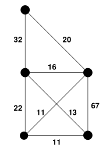
\includegraphics[width=0.5\textwidth]{Graph_1.png}
\caption{Beispielbild}
\label{fig:example}
\end{figure}
\subsection{Tabelle}
\begin{tabular}{l|c|r}
One & Two & Three\\\hline
33 & G & 55\\
\end{tabular}\\
\begin{table}
\begin{tabular}{l|p{6cm}|r}
One & Two & Three\\\hline
33 & G & 55\\
\end{tabular}
\caption{Tabelle}
\label{tab:table1}
\end{table}
\label{Sourcecode}
\subsection{Direkt im Dokument}
\begin{lstlisting}
#include <stdio.h>
/**
* main function
* prints a "Hello World"
*/

int main(int argc, char** argv)
{
	printf("Hello World\n");
	return 0;
}
\end{lstlisting}	

\end{document}